%! TEX root = ./main.tex

\section{Perception}
\begin{itemize}
    \item Raw Data $\implies$ Features $\implies$ Objects $\implies$ Places/Situations
\end{itemize}

\subsection{Sensors}
\subsubsection{Types of Sensors}
\begin{itemize}
    \ides{Proprioceptive (PC):} Measure values internally to the system
    \ides{Exteroceptive (EC):} Acquire information about the robots environment
    \ides{Passive (P):} Measure ambient environmental energy
    \ides{Active (A):} Emit energy into the environment and measure the environments reaction to it
        \begin{itemize*}
            \ipro More accurate
            \icon May interfere
            \icon May affect the characteristic one wants to measure
        \end{itemize*}
    \ides{Common Sensors}
        {\scriptsize
        \begin{tabular}{l l l}
            Sensor Type & System & Class\\\hline
            Tactile & Bumpers & EC, P \\
            Wheel/motor & Brush encoders & PC, P \\
            & Optical encoders & PC, A \\
            Heading & Compass & EC, P \\
            & Gyroscope & PC, P \\
            & Inclinometer & EC, A/P \\
            Acceleration & Accelerometer & PC, P \\
            Beacons & GPS & EC, A \\
                & Radio, ultrasonic, & EC, A \\
                & Reflective Beacons \\
            Motion/speed & Doppler: radar/sound & EC, A \\
            Range & Ultrasound, laser, & EC, A \\
                & struct. light, ToF \\
            Vision & CCD/CMOS & EC, P
        \end{tabular}}
    \ides{Encoders:}
        \begin{itemize*}
            \item Convert linear/angular motion of a shaft to digital
            \item For control of motor-driven joints
        \end{itemize*}
    \ides{Heading Sensors:}
        \begin{itemize*}
            \item Determine orientation and inclination w.r.t some reference
            \ides{Gyroscope:}
                \begin{itemize*}
                    \item Absolute measure for heading
                    \ides{Mechanical:} Fast spinning wheel
                    \ides{Optical:} Laser beam in fiber coil; Measure phase shift
                \end{itemize*}
        \end{itemize*}
    \ides{Range Sensors:}
        \begin{itemize*}
            \item Traveled distance $d$ of a sound or electromagnetic wave after a \textbf{time of flight} $t$
            \item $d=ct$
            \item Sound: $c = 0.3\,\mathrm m / \mathrm{ms}$
            \item Light: $c = 0.3\,\mathrm m / \mathrm{ns}$
        \end{itemize*}
    \ides{GPS:}
        \begin{itemize*}
            \item Satellites send their position and time to the device
            \item Device computes location based on ToF
            \item Time synchronisation and measurement is critical
            \ides{RTK:} Measure of carrier wave phase - up to centimeter-level accuracy
        \end{itemize*}
    \todo{More Sensors?}
\end{itemize}

\subsubsection{Uncertainty Representation}
\begin{itemize}
    \ides{Systematic Error:}
        \begin{itemize*}
            \item Deterministic
            \item Can be modelled and calibrated
        \end{itemize*}
    \ides{Random Error:}
        \begin{itemize*}
            \item Cannot be predicted
            \item Described statistically
        \end{itemize*}
    \item Density function identifies for each possible $x$ of RV $X$ a probability $f(x)$
        \begin{itemize*}
            \item $\int_{-\infty}^\infty f(x) \rmd x = 1$
            \item $\mu = E[X] = \int_{-\infty}^\infty x f(x) \rmd x$
            \item $\sigma^2 = E[(X - E[X])^2]$
        \end{itemize*}
    \ides{Error Propagation Law}
        \begin{itemize*}
            \item Error propagation in system with $n$ inputs and $m$ outputs $f: \R^n \to \R^m$, $f: X_1, \dots X_n \mapsto f(X_1, \dots, X_n) = Y_j$
            \item Uncertainty of $X_i$ is known
            \item Mapping between input covariance $C_X$ and output covariance $C_Y$: $C_Y = F_X C_X F_X^\transpose$
            \item $F_X = \bigtriangledown f_X =
                \begin{bmatrix}
                    \frac{\partial f_1}{\partial X_1} & \dots & \frac{\partial f_1}{\partial X_n}\\
                    \vdots & \ddots & \vdots\\
                    \frac{\partial f_m}{\partial X_1} & \dots & \frac{\partial f_m}{\partial X_n}
                \end{bmatrix}$
            \ides{$\mathbf{C_{X/Y}}$:} Covariance of input uncertainties/propagated uncertainties of the output
        \end{itemize*}
\end{itemize}

\subsection{Computer Vision}

\subsubsection{Camera Model}
\begin{itemize}
    \ides{Pinhole Model:}
        \begin{itemize*}
            \item Black box with single hole
            \item Beam of rays enter through the \textbf{Optical Center/Center of Projection C}
            \item Inverted image is projected onto the \textbf{Image Plane}
        \end{itemize*}
    \ides{Converging Lens:}
        \begin{itemize*}
            \item Focuses multiple rays from the same point on the object to the same point on the image plane
            \item All rays parallel to the \textbf{optical axis} converge at the \textbf{focal point}
            \item Rays passing through the \textbf{optical center} are not diverged
        \end{itemize*}
    \\ \begin{minipage}[b]{0.49\linewidth}
        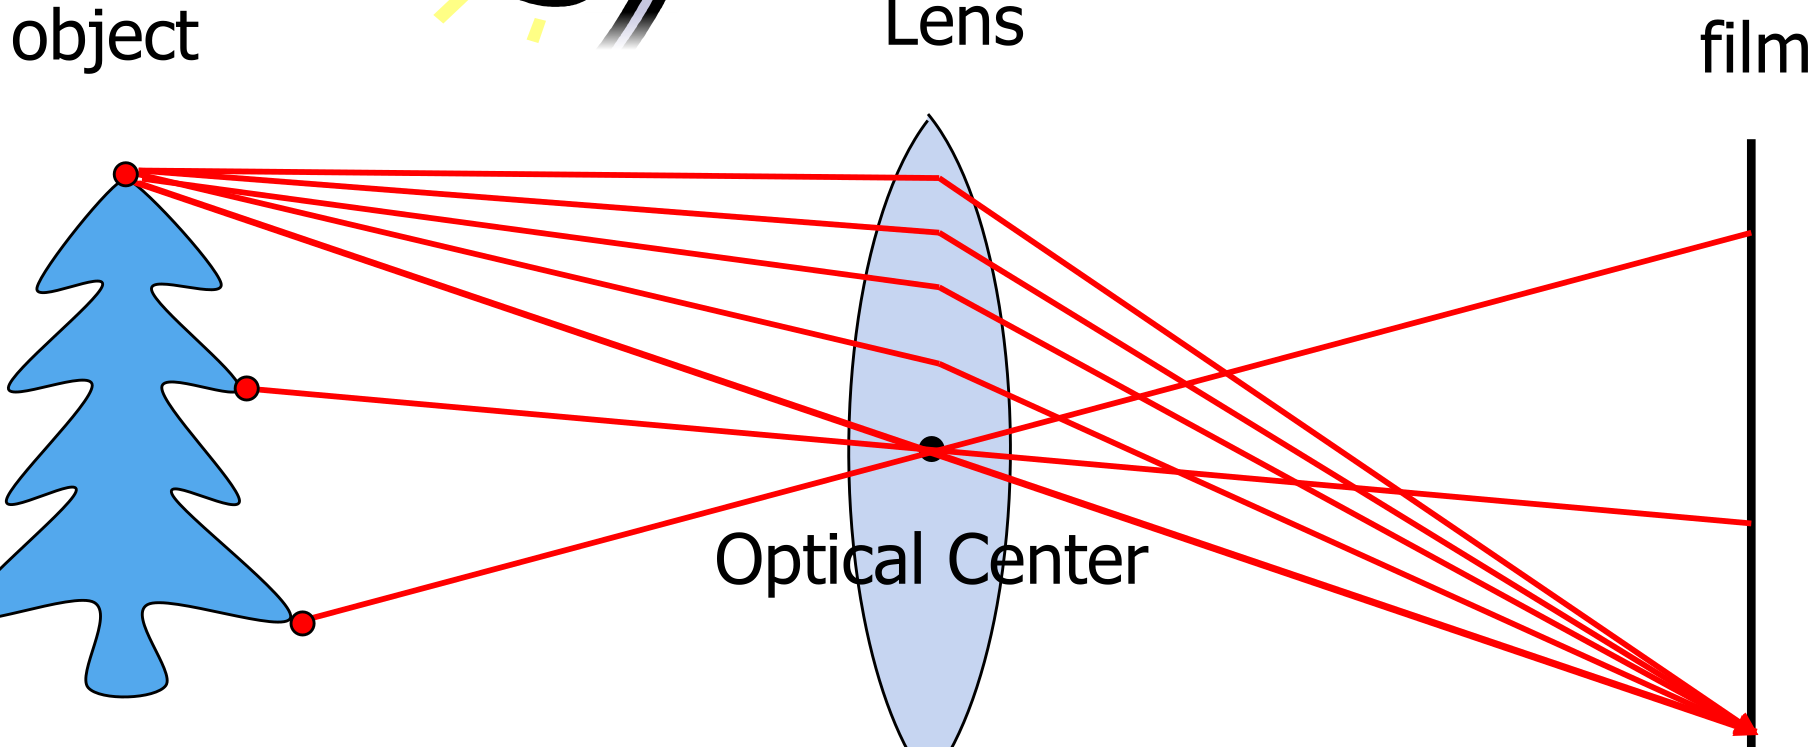
\includegraphics[width=\linewidth]{./Figures/04_Lens1.png}
    \end{minipage}
    \begin{minipage}[b]{0.49\linewidth}
        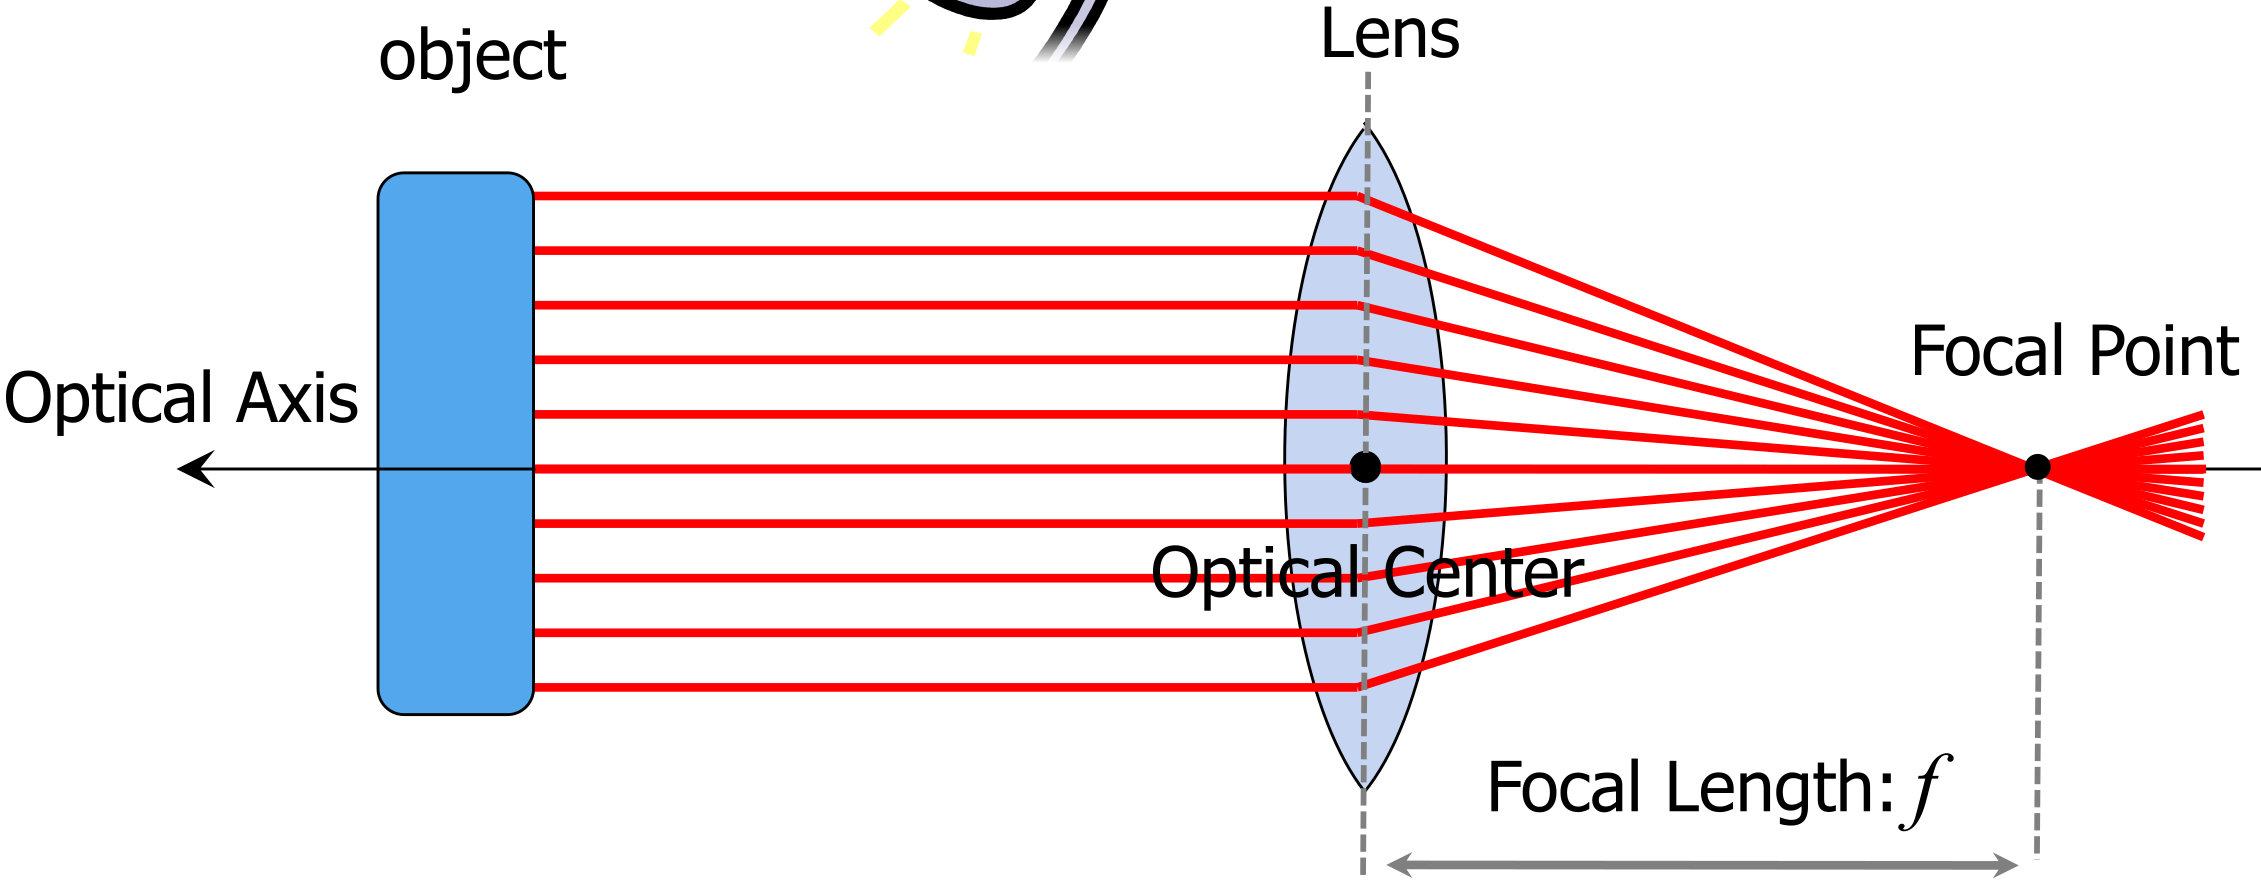
\includegraphics[width=\linewidth]{./Figures/04_Lens2.png}
    \end{minipage}
    \ides{Thin Lens equation:} $\frac{1}{f} = \frac{1}{z} + \frac{1}{e}$
    \ides{Pinhole Approximation:} $z \gg f \implies f \approx e$
        \begin{itemize}
            \item I.e. lens is approximated as pinhole at distance $f$ from image plane
            \item If follows that $B' = \frac{f}{z}B$
        \end{itemize}
    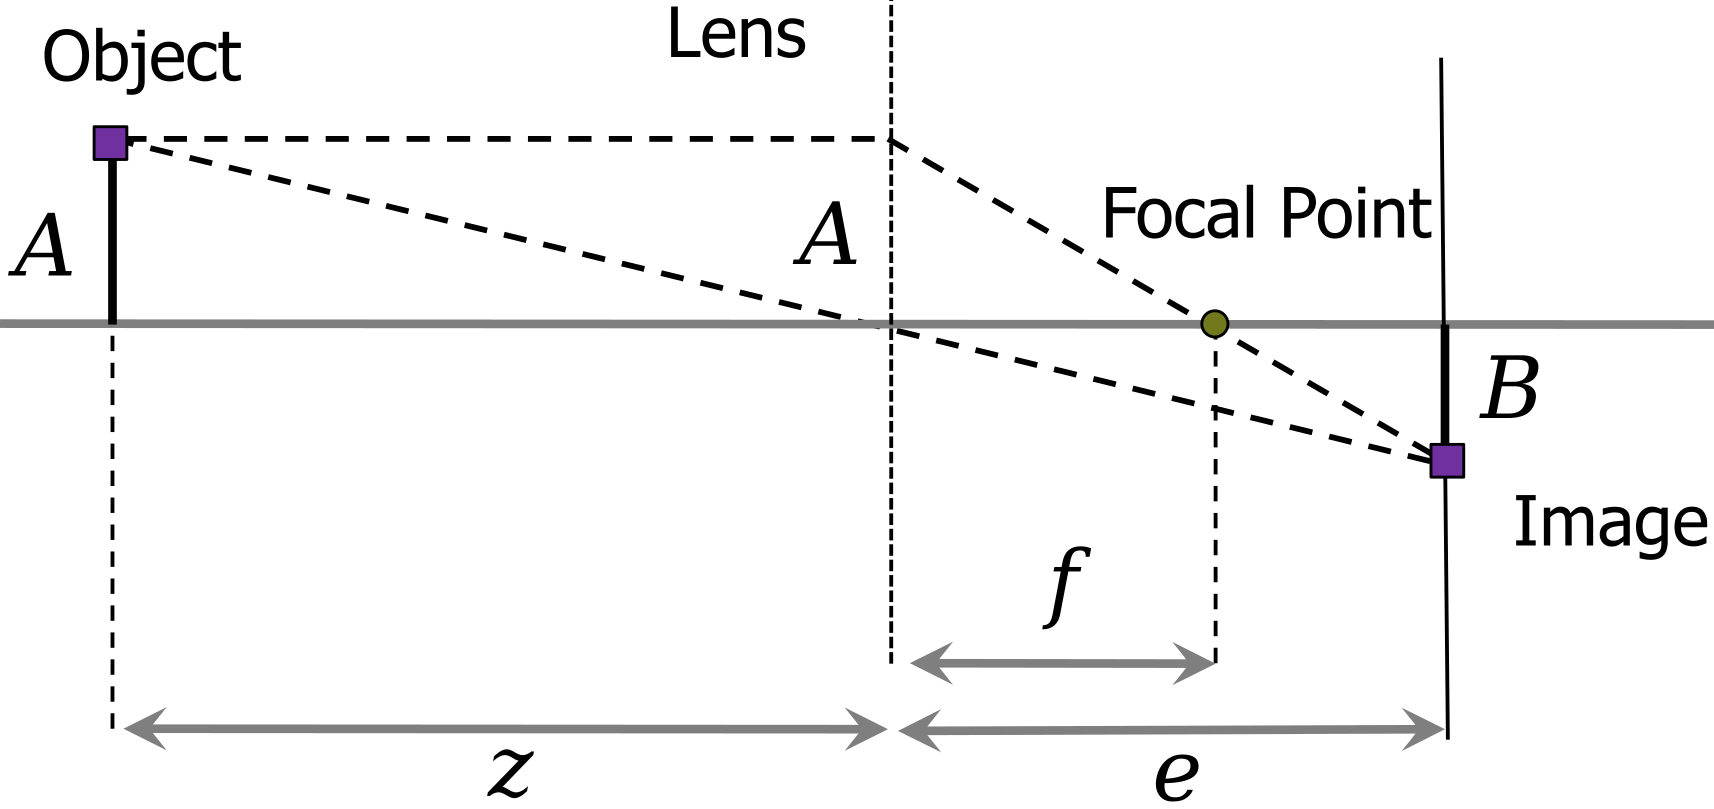
\includegraphics[width=\linewidth]{./Figures/04_ThinLensEquation.png}
\end{itemize}

\subsubsection{Perspective Camera}
\begin{itemize}
    \item Image plane represented in front of $C$
    \item Camera measures angles and not distances
    \item Project pt $P_W = (x,y,z)$ onto $p_C = (u,v)$ on the image plane
    \ides{Perspective Equations:}\\
        \begin{itemize*}
            \item $x = f \frac{X_c}{Z_C}$
            \item $y = f \frac{Y_c}{Z_C}$
        \end{itemize*}\\
        \begin{itemize*}
            \item $u = u_0 + k x$
            \item $v = v_0 + k y$
            \ides{Scale factor $k$} $[\text{pixels}/\text{meter}]$
            \ides{Focal length in pixels:} $kf = \alpha$
        \end{itemize*}
        \begin{itemize}
            \item $\implies \tilde p =
                \begin{bmatrix}
                    \lambda u\\
                    \lambda v\\
                    \lambda
                \end{bmatrix} =
                \underbrace{
                \begin{bmatrix}
                    kf & 0 & u_0\\
                    0 & kf & v_0\\
                    0 & 0 & 1
                \end{bmatrix}}_{K}
                \begin{bmatrix}
                    X_C\\
                    Y_C\\
                    Z_C
                \end{bmatrix}$
        \end{itemize}
    \ides{Intrinsic Parameter $K$:} depending on camera
    \item Rigid Body transformation\\
        $\begin{bmatrix}
            X_C\\
            Y_C\\
            Z_C
        \end{bmatrix}=
        \underbrace{
        \begin{bmatrix}
            r_{11}  & r_{12} & r_{13}\\
            r_{21}  & r_{22} & r_{23}\\
            r_{31}  & r_{32} & r_{33}\\
        \end{bmatrix}}_{R}
        \begin{bmatrix}
        X_W\\
        Y_W\\
        Z_W
        \end{bmatrix} +
        \underbrace{
        \begin{bmatrix}
            t_1\\
            t_2\\
            t_3
        \end{bmatrix}}_{T} = [R \mid T]
        \begin{bmatrix}
            X_W\\
            Y_W\\
            Z_W\\
            1
        \end{bmatrix}$
\end{itemize}
\begin{minipage}[b]{0.49\linewidth}
    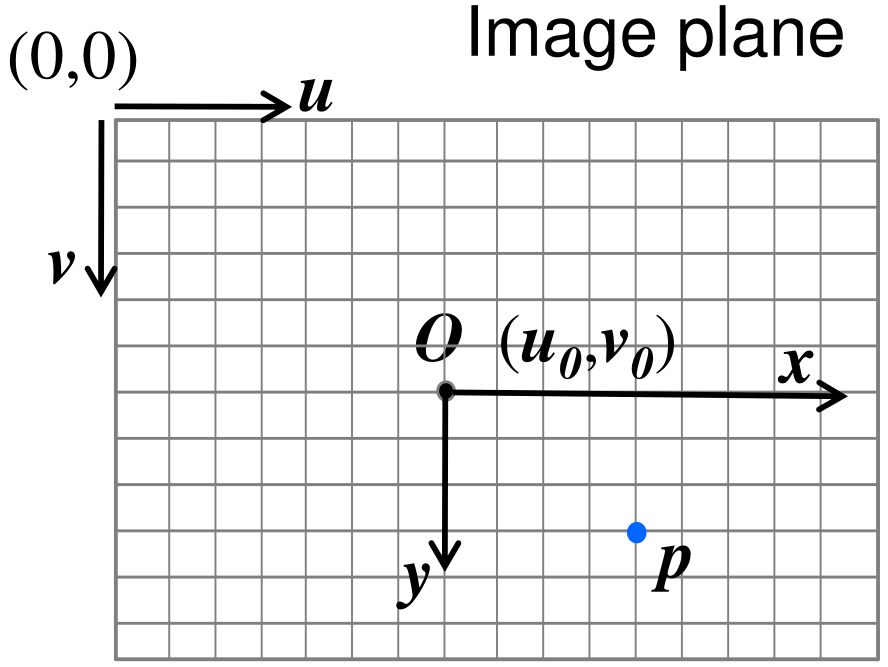
\includegraphics[width=\linewidth]{./Figures/04_PerspectiveProjection1.png}
\end{minipage}
\begin{minipage}[b]{0.49\linewidth}
    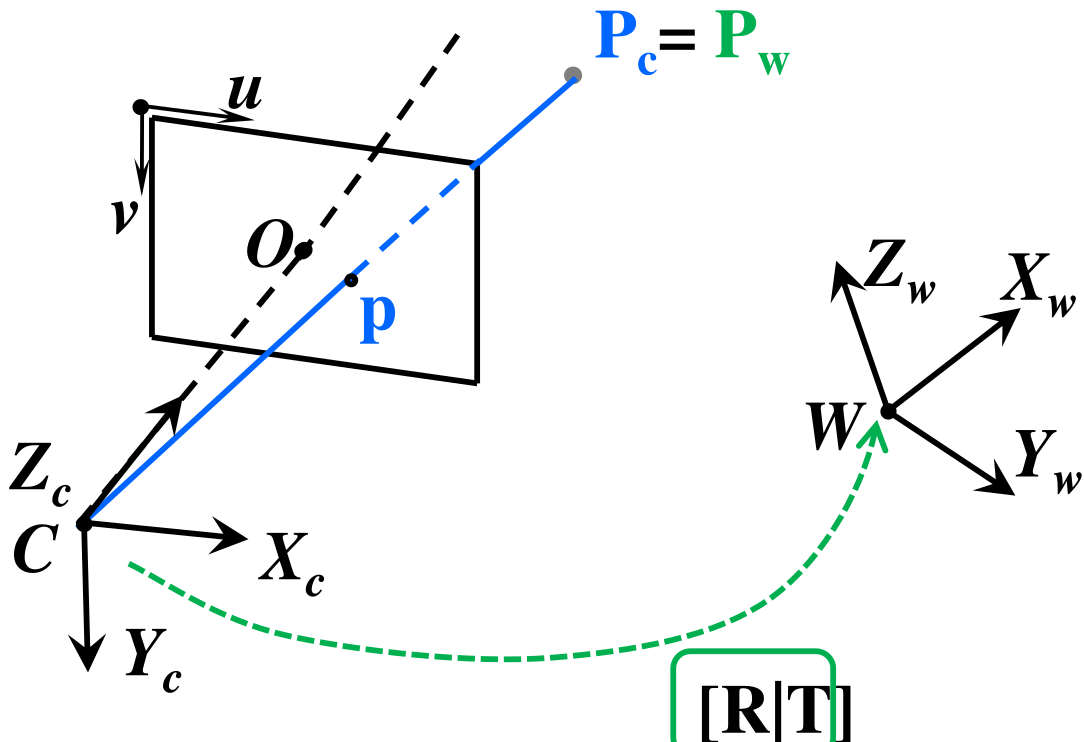
\includegraphics[width=\linewidth]{./Figures/04_PerspectiveProjection2.png}
\end{minipage}
\begin{itemize}
    \ides{Extrinsic Parameter $[R \mid T]$:} depending on transformation
    \ides{Perspective Projection:} $K[R \mid T]$
    \item $\implies \tilde p =
        \begin{bmatrix}
            \lambda u\\
            \lambda v\\
            \lambda
        \end{bmatrix} = K[R \mid T]
        \begin{bmatrix}
            X_W\\
            Y_W\\
            Z_W\\
            1
        \end{bmatrix}$
    \ides{Barrel Distortion}
        \begin{itemize}
            \item Straight lines get bend
            \ides{Barrel Distortion:} Image gets ``round''
            \ides{Pincusion Distortion:} Corners pulled out
            \item Model:
                $\begin{bmatrix}
                    u_d\\
                    v_d
                \end{bmatrix} = (1 + k_1 r^2)
                \begin{bmatrix}
                    u - u_0\\
                    v - v_0
                \end{bmatrix} +
                \begin{bmatrix}
                    u_0\\
                    v_0
                \end{bmatrix}$
                \begin{itemize}
                    \ides{Distortion Parameter $\mathbf{k_1}$:} Intrinsic parameter
                    \item $r^2 = (u - u_0)^2 + (v - v_0)^2$
                \end{itemize}
        \end{itemize}
\end{itemize}

\subsubsection{Omnidirectional Camera}
\begin{itemize}
    \ides{Dioptric:}
        \begin{itemize*}
            \item System of lenses
            \item $\sim 180^\circ$ FOV
        \end{itemize*}
    \ides{Catadioptric:}
        \begin{itemize*}
            \item Combination of lens and mirrors
            \item $> 180^\circ$ FOV
            \item Greatly distorted (can be removed depending on mirror)
        \end{itemize*}
        \begin{itemize}
            \ides{Central Camera:} Mirror shaped that all incoming rays have same \textit{single effective viewpoint}
                \begin{itemize}
                    \ides Correct mirror placement is important
                    \ipro Unwarping into perspective image possible
                    \ipro Can convert points in the image to spherical vectors
                    \ipro Can apply standard algorithms
                \end{itemize}
        \end{itemize}
    \ides{Polydioptric:}
        \begin{itemize*}
            \item Multiple cameras
            \item $\sim 360^\circ$ FOV
        \end{itemize*}
\end{itemize}

\subsubsection{Camera Calibration}
\begin{itemize*}
    \item Determine intrinsic (and extrinsic) camera parameters
    \item $\lambda
        \begin{bmatrix}
            u\\
            v\\
            1
        \end{bmatrix} = K [R|T]
        \begin{bmatrix}
            X_W\\
            Y_W\\
            Z_W\\
            1
        \end{bmatrix} \overset{!}{=} \linebreak
        \begin{bmatrix}
            m_{11} & \dots & m_{14}\\
            \vdots & \ddots & \vdots\\
            m_{31} & \dots & m_{34}
        \end{bmatrix}
        \begin{bmatrix}
            X_W\\
            Y_W\\
            Z_W\\
            1
        \end{bmatrix}$
    \item Find all $m_{ij}$
    \item Requires $\ge 6$ pts
    \item Done using least-square method
    \item Need to decompose the found matrix into $K, R, T$
    \item QR factorize $3 \times 3$ submatrix $m_{11}:m_{33} \Rightarrow K := R, R := R$
    \item Calculate $T = K^{-1}[m_14, m_{24}, m_{34}]^\transpose$
\end{itemize*}

\subsubsection{Stereo Vision}
\begin{minipage}[b]{0.49\linewidth}
    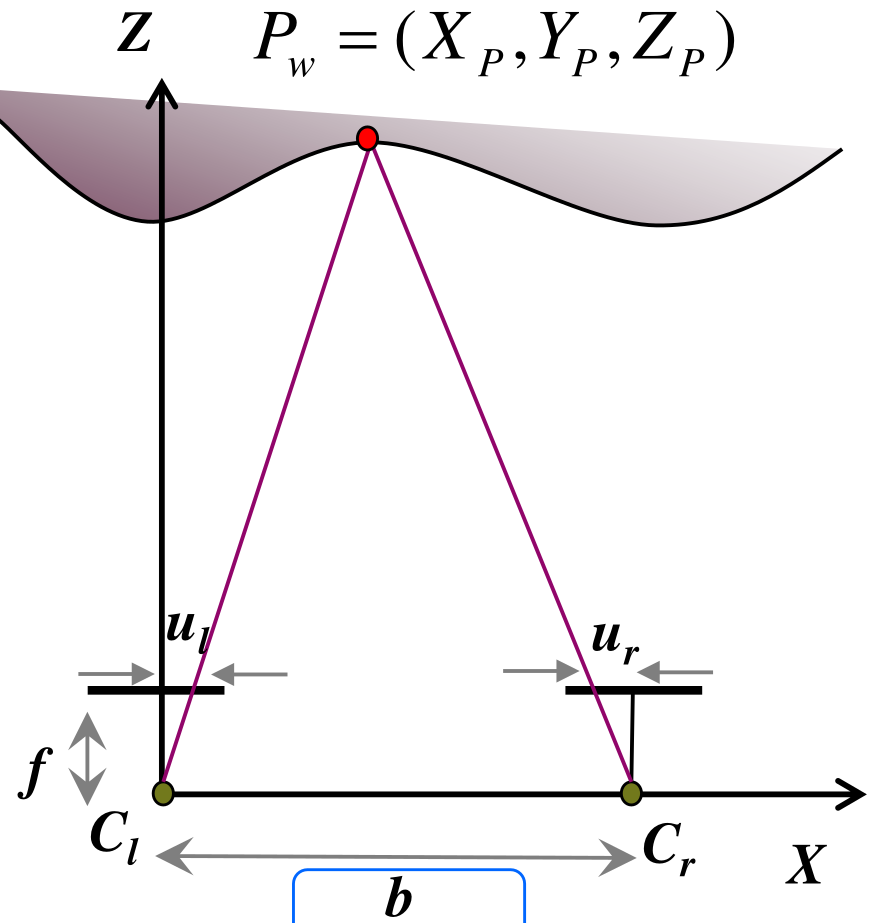
\includegraphics[width=\linewidth]{./Figures/04_StereoVision.png}
\end{minipage}
\begin{minipage}[b]{0.49\linewidth}
    \raggedright
    \begin{itemize}
        \item Obtain depth information from two cameras with know relative position
        \item Cameras need to be calibrated
        \item Calculating depth $Z_P$ of point $P_W$ (distance to $P_W$)
        \ides{Baseline $\mathbf{b}$:} Distance between the two cameras
    \end{itemize}
\end{minipage}
\begin{itemize}
    \ides{Disparity:} Difference in image location of the projection of a 3D point on the two image panes: $u_l - u_r$
    \item Two identical cameras aligned on $x$
        \begin{itemize}
            \item $Z_P = \frac{bf}{u_l - u_r}$
        \end{itemize}
    \item Two identical cameras in different Coordinate Systems
        \begin{itemize}
            \item $C_r$ is a rigid body transformation of $C_l$\\
            \item Triangulation
            \begin{itemize*}
                \item $\tilde p_l = \lambda_l
                    \begin{bmatrix}
                        u_l\\
                        v_l\\
                        1
                    \end{bmatrix} = K_l
                    \begin{bmatrix}
                        X_W\\
                        Y_W\\
                        Z_W
                    \end{bmatrix}$
                \item $\tilde p_r = \lambda_r
                    \begin{bmatrix}
                        u_r\\
                        v_r\\
                        1
                    \end{bmatrix} = K_r R
                    \begin{bmatrix}
                        X_W\\
                        Y_W\\
                        Z_W
                    \end{bmatrix} + T$
            \end{itemize*}
        \end{itemize}
    \ides{Disparity Map}
        \begin{itemize}
            \item Compute disparity for corresponding points of every pixel
            \item Can compute the depth from it and reconstruct 3D scene
        \end{itemize}
\end{itemize}

\subsubsection{Correspondence Search}
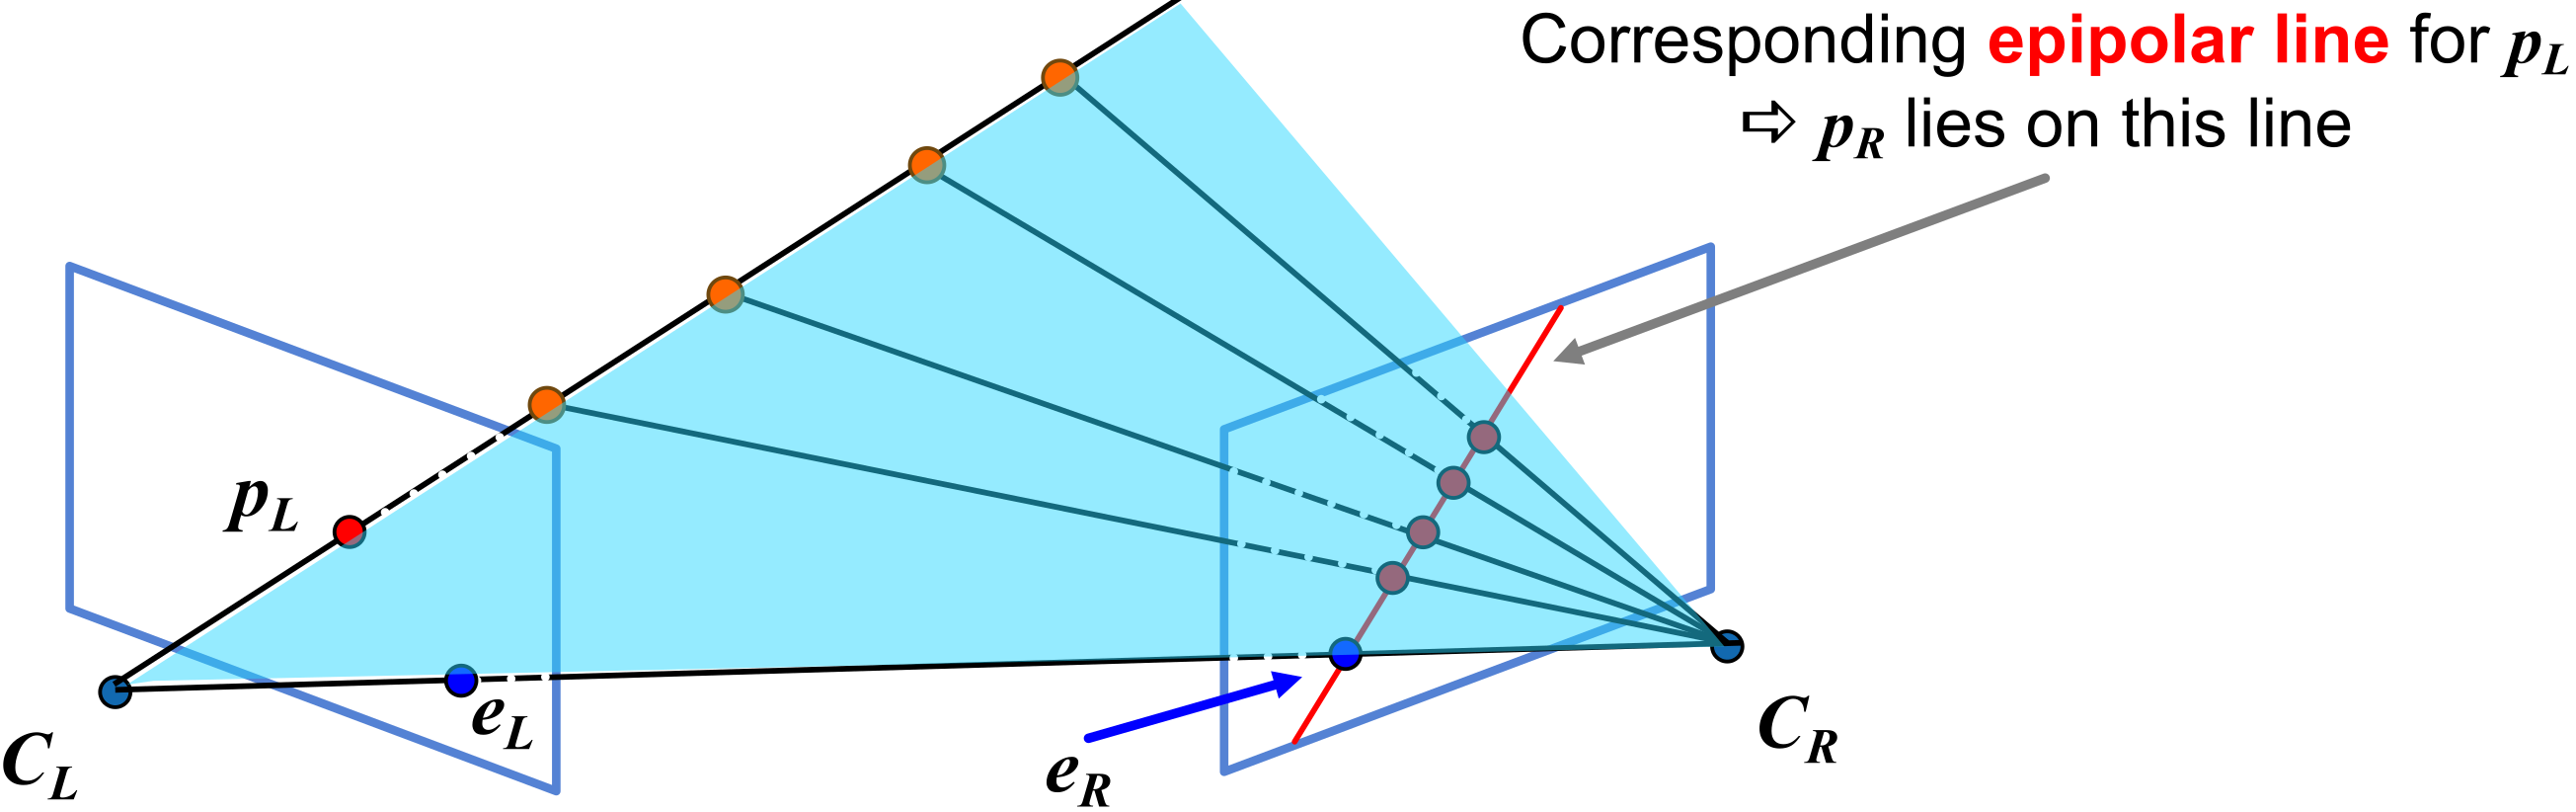
\includegraphics[width=\linewidth]{./Figures/04_EpopolarPlan.png}
\begin{itemize}
    \item Identify corresponding points in two images of the same scene
    \item Measure similarity of two pts using a similarity measurement
    \ides{Epipolar Plane:} Spanned by $C_l$, $C_r$ and some pt $P_W$
    \ides{Epipolar Line:} Projection of the ray from one camera through points in the other camera
    \ides{Epipole:} Projection of other camera in image plane
        \begin{itemize*}
            \item All epipolar lines go through it
        \end{itemize*}
    \ides{Epipolar Constraint:} Correspond of pt of left images lies on the epipolar line of the right image
    \ides{Epipolar Rectification:} Transform both images to make epipolar lines collinear and parallel:
        \begin{itemize*}
            \item[1)] Remove radial distortion
            \item[2)] \textbf{Warping:} Reprojection of both images to same plane
        \end{itemize*}
\end{itemize}

\subsubsection{Triangulation}
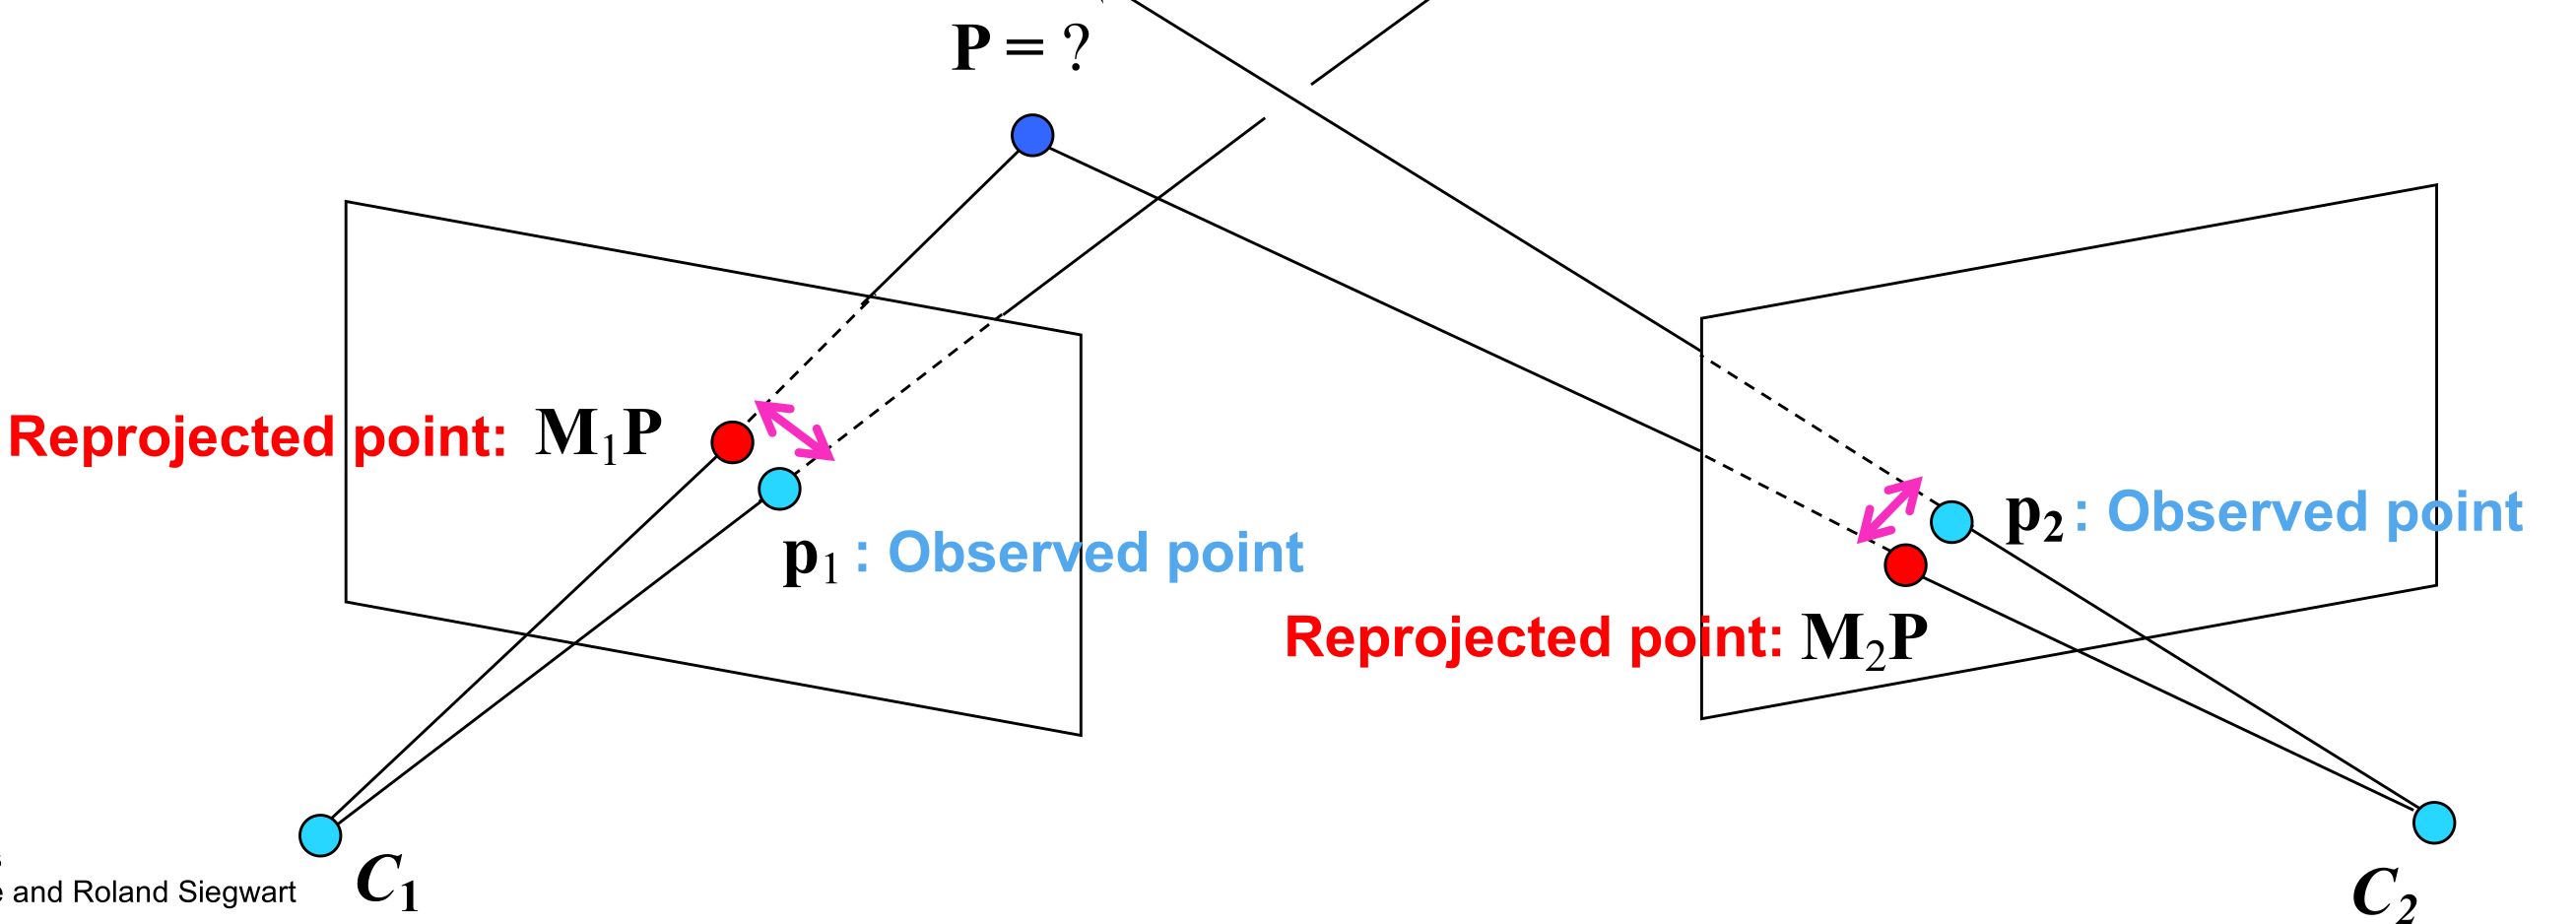
\includegraphics[width=\linewidth]{./Figures/04_Triangulation.png}
\begin{itemize}
    \item Find 3D coordinate of a point given the projections on multiple image planes
    \item $R_i, T_i, K_i$ are known
    \item
        \begin{itemize*}
            \item $\lambda_1
                \underbrace{\begin{bmatrix}
                    u_1\\
                    v_1\\
                    1
            \end{bmatrix}}_{p_1} = \underbrace{K_1[I \mid 0]}_{M_1}
                \underbrace{\begin{bmatrix}
                    X_x\\
                    Y_w\\
                    Z_w\\
                    1
                \end{bmatrix}}_{P}$
            \item $\lambda_2
                \begin{bmatrix}
                    u_2\\
                    v_2\\
                    1
                \end{bmatrix} = K_2[R \mid T]
                \begin{bmatrix}
                    X_x\\
                    Y_w\\
                    Z_w\\
                    1
                \end{bmatrix}$
        \end{itemize*}
    \item No unique solution du to noise and errors
    \ides{Linear Approach:} Solved using SVD
    \ides{Reprojection Approach:} Minimize Sum of Square Reprojection Error $\mathrm{SSRE} = \norm{P_1 - M_1 P}^2 + \norm{p_2 - M_2 P}^2$
    \item Baseline is important:
        \begin{itemize}
            \ides{Too Small:} Large depth error
            \ides{Too Large:}
                \begin{itemize*}
                    \item Objects may be visible only from one camera
                    \item Difficult search problem for close objects
                \end{itemize*}
        \end{itemize}
\end{itemize}

\subsubsection{Structure from Motion (SfM)}
\begin{itemize}
    \item Given corresponding image points $\{(u_1^i, v_1^i), (u_2^i, v_2^i)\}$, recover:
        \begin{itemize*}
            \item 3D location $P_i$ of all $n$ pts
            \item Relative pose of right camera $R, T$
            \item Camera intrinsic $K$ (optionally)
        \end{itemize*}
    \item Assume $K$ is known
    \ides{Knowns:} $4n$: $n$ correspondences
    \ides{Unknowns:} $5 + 3n$: rotation ($3$), translation ($2$, since scale cannot be recovered), $n$ 3D pts ($3n$)
    \item Solution exists iff $4n \ge 5 + 3n \implies n \ge 5$
    \ides{Crossp.:} $a \times b =
        \begin{bmatrix}
            0 & -a_z & a_y\\
            a_z & 0 & -a_x\\
            -a_y & a_x & 0
        \end{bmatrix}
        \begin{bmatrix}
            b_x\\
            b_y\\
            b_z
        \end{bmatrix} = [a]_\times b$
    \ides{Epipolar Constraint:} $p_2^T E p_1 = 0$
    \ides{Essential Matrix:} $E = [T]_\times R$
        \begin{itemize}
            \item Computed with $\ge 5$ correspondences
            \item Can be decomposed into $R$ and $T$
        \end{itemize}
    \ides{Normalized Img Coordinates:} $p = [\bar u, \bar v, 1]^\transpose = K^{-1}[u, v, 1]^\transpose$
    \ides{8-pt Algorithm}
        \begin{itemize*}
            \item Algorithm to compute essential matrix
            \item Uses $\ge 8$ pts
        \end{itemize*}
        \begin{itemize}
            \item $p_2^\transpose E p_1 = [\bar u_2, \bar v_2, 1]
                \begin{bmatrix}
                    e_11 & e_12 & e_13\\
                    e_21 & e_22 & e_23\\
                    e_31 & e_32 & e_33
                \end{bmatrix}
                \begin{bmatrix}
                    \bar u_1\\
                    \bar v_1\\
                    1
                \end{bmatrix} = 0$
            \item $\underbrace{[u_2u_1, u_2v_1, u_2, v_2u_1, v_2v_1, v_2, u_1, v_1, 1]}_{Q: \text{known}} \cdot \linebreak \underbrace{[e_{11}, e_{12}, \dots, e_{33}]}_{\text{unknown}} = 0$
            \item For $8$ non-coplanar pts, unique solution is given by the EV of $Q$ corresponding to the smallest Eigenvalue
        \end{itemize}
\end{itemize}

\subsubsection{Image Filtering}
\begin{itemize}
    \ides{Linear:} Replace each pixel by a linear combination of its neighbours
    \ides{Shift-Invariant:} Same operation is performed on every point on the image
    \ides{Filter $\mathbf{H}$:} aka. \textit{kernel, mask, window}
    \ides{Boundaries:} Need to handle specially:
        \begin{itemize*}
            \item Ignore
            \item Zero padding
            \item Pad with edge value
            \item Mirror boundary
            \item Wrap around from other side
        \end{itemize*}
    \ides{Normalization:} Prevent img from getting brighter/darker
    \ides{Correlation:} $J(x) = F \circ I(x,y) = \sum_{i=-N}^N \sum_{j=-M}^M F(i,j) I(x + i, y + j)$
        \begin{itemize}
            \item Not associative
        \end{itemize}
    \ides{Convolution:} $J(x) = F \ast I(x,y) = \sum_{i=-N}^N \sum_{j=-M}^M F(i,j) I(x - i, y - j)$
        \begin{itemize}
            \item Equivalent to correlation except that the filter is flipped before correlating
            \item Same result to correlation if the filter is symmetric
            \item Is associative: $F \ast (G \ast I) = (F \ast G) \ast I$
        \end{itemize}
    \ides{Correlation Cost: (per pixel)}
        \begin{itemize}
            \ides{2D:}
                \begin{itemize*}
                    \ides{Mult.:} $(2N + 1)^2$
                    \ides{Add.:} $(2N - 1)^2 - 1$
                \end{itemize*}
            \ides{$\mathbf{2 \times 1D}$:}
                \begin{itemize*}
                    \ides{Mult.:} $2(2N + 1)$
                    \ides{Add.:} $4N$
                \end{itemize*}
            \ides{$\mathbf{2 \times 1D}$ with const.:}
                \begin{itemize*}
                    \ides{Mult.:} $1$
                    \ides{Add.:} $4N$
                \end{itemize*}
        \end{itemize}
    \ides{Derivation:} $J(x) = \frac{I(x+1)-I(x-1)}{2}$
    \ides{Smoothing:}
        \begin{itemize}
            \item For blurring or noise detection
            \ides{1D Gaussian:} $G_\sigma(x) = \frac{1}{\sigma \sqrt{2 \pi}} \mathrm e^{-\frac{x^2}{2 \sigma^2}}$
            \ides{2D Gaussian:} $G_\sigma(x, y) = \frac{1}{2 \pi \sigma^2} \mathrm e^{-\frac{x^2 + y^2}{2 \sigma ^2}} = g_\sigma(x) \cdot g_\sigma(y) =
                \tfrac{1}{\sigma \sqrt{2\pi}} \mathrm e^{\frac{-x^2}{2\sigma^2}}
                \cdot
                \tfrac{1}{\sigma \sqrt{2\pi}} \mathrm e^{\frac{-y^2}{2\sigma^2}}$
                \begin{itemize}
                    \item Is separable
                \end{itemize}
        \end{itemize}
    \ides{Similarity Measure}
        \begin{itemize}
            \ides{Sum of Square Diff.:} $\mathrm{SSD}(x) =
                \sum_i (F(i) - I(x+i))^2 =
                \sum_i F(i)^2 + \sum_i I(x+i)^2 - 2 \sum_i (F(i) I(x+i))$
            \ides{Normalized Cross Correlation:} $\mathrm{NCC} =
                \frac{\sum_i (F(i)I(x + i))}
                {\sqrt{\sum_i F(i)^2} \sqrt{\sum_i I(x+i)^2}}$
            \ides{Zero-Mean Normalized Cross Correlation (ZNCC)}: Invariant to local average intensity. Maximize: $\mathrm{ZNCC}(x) =
                \frac{\sum_i (F(i)- \mu_F)(I(x + i) - \mu_{I_x})}
                {
                    \sqrt{\sum_i (F(i) - \mu_F)^2}
                    \sqrt{\sum_i (I(x+i) - \mu_{I_x})^2}
                }$
                \begin{itemize*}
                    \item $\mu_F = \frac{\sum_i F(i)}{2N + 1}$
                    \item $\mu_{I_x} = \frac{\sum_i I(x+i)}{2N + 1}$
                \end{itemize*}
        \end{itemize}
    \ides{Template Matching:} Use template as filter and apply similarity measure
    \ides{Edge Detection:}
        \begin{itemize*}
            \item[1)] Noise reduction
            \item[2)] Gradient $S^\prime = (G_\sigma \ast I)^\prime = G_\sigma^\prime \ast I$
            \item[3)] Thresholding
            \item[4)] Non-maximal suppression
        \end{itemize*}
        \begin{itemize}
            \ides{Derivation of Gaussian:} $G_\sigma^\prime(x, y) = \frac{\partial G_\sigma(x, y)}{\partial x} + \frac{\partial G_\sigma(x, y)}{\partial y}$
                \begin{itemize*}
                    \item Edges at min/max
                \end{itemize*}
            \ides{Laplacian of Gaussian:} $\mathrm{LoG} = G_\sigma^{\prime\prime}(x, y) = \frac{\partial^2 G_\sigma(x, y)}{\partial x^2} + \frac{\partial^2 G_\sigma(x, y)}{\partial y^2}$
                \begin{itemize*}
                    \item Edges at zero crossing
                \end{itemize*}
            \ides{Prewitt:}
                \\ \begin{itemize*}
                    \item $F_x = \left[
                        \begin{array}{c | c | c}
                            -1 & 0 & 1\\
                            -1 & 0 & 1\\
                            -1 & 0 & 1
                    \end{array} \right]$
                    \item $F_x = \left[
                        \begin{array}{c | c | c}
                            1 & 1 & 1\\
                            0 & 0 & 0\\
                            -1 & -1 & -1
                    \end{array} \right]$
                \end{itemize*}
            \ides{Sobel:}
                \\ \begin{itemize*}
                    \item $F_x = \left[
                        \begin{array}{c | c | c}
                            -1 & 0 & 1\\
                            -2 & 0 & 2\\
                            -1 & 0 & 1
                    \end{array} \right]$
                    \item $F_x = \left[
                        \begin{array}{c | c | c}
                            1 & 2 & 1\\
                            0 & 0 & 0\\
                            -1 & -2 & -1
                    \end{array} \right]$
                \end{itemize*}
            \ides{Roberts:}
                \begin{itemize*}
                    \item $F_x = \left[
                        \begin{array}{c | c}
                            0 & 1\\
                            1 & 0\\
                    \end{array} \right]$
                    \item $F_x = \left[
                        \begin{array}{c | c}
                            1 & 0\\
                            0 & 1\\
                    \end{array} \right]$
                \end{itemize*}
        \end{itemize}
\end{itemize}

\subsubsection{Point Features}
\begin{itemize}
    \ides{Harris Corner Detection:} Patch at $(x,y)$ of size $P$ has great difference to all surrounding patches $(x + \Delta x, y + \Delta y)$
        \begin{itemize}
            \item $\mathrm{SSD}(\Delta x, \Delta y) = \sum_{x,y \in P}(I(x,y) - I(x + \Delta x, y + \Delta y))^2$
            \item $\Rightarrow \mathrm{SSD}(\Delta x, \Delta y) \approx \sum_{x,y \in P}(I_x(x,y)x - I_y(x, y)y)^2$
                \\ \begin{itemize*}
                    \item $I_{x} = \frac{\partial I(x,y)}{\partial x}$
                    \item $I_{y} = \frac{\partial I(x,y)}{\partial y}$
                    \item Using first-order Taylor approx
                \end{itemize*}
            \item $\Rightarrow \mathrm{SSD}(\Delta x, \Delta y) \approx [\Delta x, \Delta y]M[\Delta x, \Delta y]^\transpose$
                \\ \begin{itemize*}
                    \item $M = \sum_{x,y \in P}
\begin{bmatrix}
    I_x^2 & I_xI_y\\
    I_xI_y & I_y^2
\end{bmatrix} = R^{-1}
\begin{bmatrix}
    \lambda_1 & 0\\
    0 & \lambda_2
\end{bmatrix} R$
                \end{itemize*}
            \item \begin{itemize*}
                \ides{$\mathbf{\lambda_1, \lambda_2}$ small:} Flat region
                \ides{$\mathbf{\lambda_1 >> \lambda_2}$:} Edge
                \ides{$\mathbf{\lambda_1 << \lambda_2}$:} Edge
                \ides{$\mathbf{\lambda_1, \lambda_2}$ large:} Corner
            \end{itemize*}
            \ides{Cornerness Function:} $C = \text{det} - \kappa \ \text{trace}^2(M)$
                \\ \begin{itemize*}
                    \item Extract local minima
                    \item Used since calculating eigenvalues is expensive
                    \item $\kappa$ is magic number
                \end{itemize*}
            \ides{Invariant to:}
                \begin{itemize*}
                    \item Rotation
                    \item Linear intensity change
                \end{itemize*}
            \ides{Not invariant to:} Scale change
        \end{itemize}
    \ides{Scale Invariant Feature Transform (SIFT) Features:}
        \begin{itemize}
            \item Detect blobs
            \item Assigns each keypoint a orientation and descriptor
            \ides{Keypoint Detection:}
                \begin{itemize*}
                    \item[1)] Downscale image multiple times
                    \item[2)] Gaussian blur each at different rates
                    \item[3)] Calculate \textit{Difference of Gaussian (DoG)} (subtract successive smoothed images)
                    \item[4)] Find keypoints (local extrema in the DoG)
                \end{itemize*}
            \ides{Keypoint Orientation:}
                \begin{itemize*}
                    \item[1)] Generate gradient orientation histogram for each keypoint
                    \item[2)] Orientation is value of highest peak in histogram
                \end{itemize*}
            \ides{Keypoint Descriptor:}
                \begin{itemize*}
                    \item[1)] Divide neighbourhood into $4 \times 4$ regions
                    \item[2)] Compute orientation histograms along $8$ orientations
                    \item[3)] Concatenate $4 \times 4 \times 8 = 128$ values in vector
                \end{itemize*}
            \ipro High robustness
            \ipro Invariant to rotation
        \end{itemize}
    \ides{Features from Accelerated Segment Test (FAST) Detector:}
        \begin{itemize*}
            \item Detects corners
            \item Look at $16$ pixels around target pixel
            \item If they are all significantly darker/brighter, we have a FAST corner
            \ipro Fast
            \icon Not robust against noise
        \end{itemize*}
    \ides{Binary Robust Independent Elementary Features (BRIEF) Descriptor:}
        \begin{itemize}
            \item Detect blobs
                \begin{itemize*}
                    \item[1)] ``Random'' (predefined) selection of pixel pairs
                    \item[2)] Compare intensity of pairs and store result in descriptor
                    \item[3)] Matching done with Hamming Distance
                \end{itemize*}
            \ipro High speed in description and matching
            \icon Not scale invariant
            \icon Not rotation invariant
        \end{itemize}
    \ides{Binary Robust Invariant Scalable Keypoints (BRISK) Detector}
        \begin{itemize*}
            \item Detect blobs
            \item[1)] Detect corners using FAST
            \item[2)] Compare intensity similar to BRIEF but in some specific geometric pattern
            \ipro High speed
            \ipro Rotation and scale invariant
            \icon Slower than BRIEF
        \end{itemize*}
\end{itemize}

\subsubsection{Place Recognition}
\begin{itemize}
    \item Training set of images needed to create structure
    \ides{Bag of features:} Bag of descriptors of a word
        \begin{itemize*}
            \item Image is described by this set
            \item Sectional information is removed
        \end{itemize*}
    \ides{Visual Word:} Single number representing a high-dimensional descriptor
        \begin{itemize*}
            \item Done by \textbf{k-means clustering}
            \item Bag of features $\Rightarrow$ bag of visual words
        \end{itemize*}
    \ides{Visual Vocabulary:} DB of visual words created by many training images
    \item Scene is collection of visual words
    \item Efficiently find matches:
        \begin{itemize}
            \ides{Vocabulary Tree:} Hierarchical arrangement of visual vocabulary (I guess)
                \begin{itemize*}
                    \item Leaf holds image which matches the feature
                    \item By feeding in features of new images, we get a bag of matching images
                    \item Number of matches determines the probability
                \end{itemize*}
            \ides{Inverted File DB:}
                \begin{itemize*}
                    \item List of all possible visual words points to list containing all images containing this feature
                    \item Query DB for all features of a given list and count occurrences of a certain image (using voting array)
                \end{itemize*}
        \end{itemize}
    \ides{Term Frequency-Inverse Document Frequency (tf-idf):} Not all words are equally important
        \begin{itemize}
            \item Measure importance of visual word inside image
            \item Used for voting array
            \item For word $w_i$ in img $j$:
                \begin{itemize*}
                    \item $\text{tf-ids}_{ij} = \mathrm{tf}_{ij} \cdot \mathrm{idf}_i$
                    \item $\mathrm{tf}_{ij} = \frac{\# \text{occur. of } w_i \text{in } j}{\# \text{words in } j}$
                    \item $\mathrm{idf}_{i} = \log \frac{|\text{Img}|}{|\{\text{img} \mid w_i \in \text{img}\}|}$
                \end{itemize*}
        \end{itemize}
    \ides{FABMAP}
        \begin{itemize*}
            \item Place recognition
            \item Assume: worlds is set of discrete places
            \ides{Place:} vector of visual words at that scene
            \item Calculate probability of being at a know location
            \item Frequent occurring objects are suppressed
            \ipro High performance
        \end{itemize*}
\end{itemize}

\subsubsection{Line Extraction}
\begin{itemize}
    \ides{Task:} Given set of pts, find best fitting line
        \begin{itemize*}
            \item Do not have to figure out which pts belong to which line
        \end{itemize*}
    \ides{Split-and-Merge:}
        \begin{itemize}
            \item[1)] \textbf{Split:}
                \begin{itemize*}
                    \item[a)] Fit line through point set (or take end-pts)
                    \item[b)] Find most distant pt
                    \item[c)] If distance $>$ threshold, split set and repeat
                \end{itemize*}
            \item[2)] \textbf{Merge:} If two consecutive line segments are almost collinear, merge them
            \icon Sensitive to outliers
        \end{itemize}
    \ides{Random Sample Consensus (RANSAC):}
        \begin{itemize*}
            \item[1)] Draw line through two randomly selected pts
            \item[2)] Compute distance of all pts to it
            \item[4)] Repeat $k = \frac{\log({1 - p)}}{\log(1 - w^2)}$ times
                \begin{itemize*}
                    \ides{w:} fraction of inliers
                    \ides{p:} prob of finding set of pts free of outliers
                \end{itemize*}
            \item[5)] Select line with least total error
        \end{itemize*}
        \begin{itemize}
            \icon Non-Deterministic
        \end{itemize}
    \ides{Hough-Transform:}
        \begin{itemize}
            \item Each pt in image space defines a sinosoid in Hough space
        \end{itemize}
        \begin{itemize*}
            \item[1)] For each pt compute $\rho = x \cos \theta + y \sin \theta, \theta \in [0, 180]$
            \item[2)] Capture votes for parameters
            \item[3)] Find $(rho, \theta)$ with most votes
        \end{itemize*}
\end{itemize}
